\documentclass[../main.tex]{subfiles}
\graphicspath{{\subfix{../images/}}}
\begin{document}

\begin{figure}[h!]
    \centering
    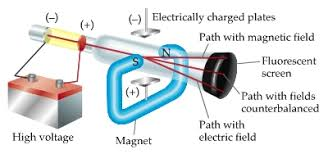
\includegraphics[scale=0.9]{images/08.JJ-Thomson..jpg}
    \caption{Autre schéma réaliste}
    \label{fig:my_label}
\end{figure}

\section{Déroulement de l'expérience}
\begin{enumerate}[I]
    \item \textbf{Le but de l'expérience de J.J. Thomson :}
    \begin{enumerate}[A.]
        \item savoir la polarité des rayons cathodiques découvert avant par Hertz
    \end{enumerate}
    \item \textbf {La théorie :}
    \begin{enumerate}[A.]
        \item formule de l'énergie mécanique (incluant l 'énergie cinétique et celle de l'énergie potentielle)
        \item champs magnétiques et électriques
        \item électricité (loi de Coulomb) 
    \end{enumerate}
    \item \textbf {Les hypothèses de départ :}
    \begin{enumerate}[A.]
        \item Il peut y avoir ou non des champs électriques ou magnétiques au niveau des 2 plaques métalliques.
        \item Le voltage du générateur est très élevé.
        \item Les plaques métalliques sont chargées.
        \item Le tube cathodique est étanche et a été mis partiellement sous vide (vidé partiellement de son air).
        \item L'écran est composé d'une couche de phosphore.
    \end{enumerate}
    \item \textbf{La marche à suivre :}
    
    \begin{enumerate}[A. ]
        \item On voit, dans le dispositif ci-dessus, un générateur branché à une cathode et à une anode.
        \item Ce générateur va, comme son nom l'indique d'ailleurs, générer/créer des électrons.
        \item S'il n'y avait pas le tube, ses électrons formeront une boucle infinie, en passant sans cesse par la borne positive et par la borne négative. 
         \item Quand il y a un potentiel électrique assez élevé entre la cathode et l'anode, des rayons cathodiques partent de la cathode(d'où vient leur nom).
         \item On va créer une haute tension avec le générateur.
        \item Ces rayons sont de plus en plus fins, au fil de leur parcours donc en traversant l'anode et la fente, qui se situe avant les plaques métalliques, mais qui est quand même dans le même secteur que la cathode et l'anode.
        \item Ils auront beaucoup d'énergie du fait du haut voltage qu'a le générateur, ils vont donc aller à une vitesse assez élevée.
        \item Les électrons passent ensuite dans le tube et continuent jusqu'aux deux plaques métalliques.
        \item Celle du dessus est chargée négativement et celle du dessous est chargée positivement.
        \item Les rayons cathodiques vont alors dévier vers le haut, attirés par le positif, si on change la polarité des deux plaques, ils seront déviés vers le bas.
        \item Il y a un aimant en forme de O coupé au milieu par le tube, qui se situe à l'extérieur du tube, de part et d'autre à celui-ci.
        \item On a pu constater que le champ magnétique produit par les 2 aimants faisaient également dévier les rayons cathodiques.
        \item Sur l'écran fluorescent, il y a des mesures qui relèvent de où a tapé le faisceau cathodique. 
        \item Chaque fois que le faisceau touche l'écran, celui-ci s'illumine d'une tache lumineuse.
        \item C'est le principe du phosphore.
        \item Comme paramètre de l'expérience, il a choisit les plaques métalliques, dont il changeait la matière pour voir si les rayons cathodiques avaient toujours le même comportement.
    \end{enumerate}
    \item \textbf{Les mesures :}
    \begin{enumerate}
        \item Comme mesures, J.J. Thomson a mesuré le voltage du générateur.
        \item Il a aussi pris note, grâce ses graduations sur l'écran fluorescent, de là où arrivait le faisceau cathodique.
        \item Et de ces mesures, il a obtenu des résultats que satisfaisants.
    \end{enumerate}
    \item \textbf {Les résultats :}
    \begin{enumerate}
        \item Il a obtenu le rapport de la charge à la masse, chose qui n'a jamais été trouvé avant lui.
        \item Cela lui a permis notamment de trouver l'existence de petites particules chargées négativement qui se trouve dans l'atome. 
    \end{enumerate}
    \item \textbf {La conclusion :}
    \begin{enumerate}
        \item Dans l'atome, il existe des petites particules chargées négativement, en orbite autour du noyau : les électrons.
        \item On a trouvé le rapport charge et masse de l'électron, chose jamais faite avant.
        \item Le fait de baisser la pression du tube, donc de le mettre partiellement sous vide s'avère légitime.
        \item En effet, Hertz, un autre scientifique a effectué la même expérience un peu avant Thomson et n'avait pas observé de déviation du faisceau et a donc dit qu'il n'y avait pas de champ électrique produit par les plaques, mais Thomson en baissant la pression a constaté que le faisceau déviait de plus en plus, attiré par la plaque positive.
        \item D'où il a conclut que le faisceau devait être négatif.
        \item En connaissant le rapport charge et masse, il a constaté que la masse était nettement plus petite qu'un atome d'hydrogène (atome le plus petit), il en a donc conclut que la particule qu'il venait de découvrir devait se trouver à l'intérieur de l'atome.
        \item En changeant plusieurs fois la matière des plaques métalliques, Thomson a pu conclure que l'expérience marchait pour n'importe quelle matière, c'était donc un cas général de la matière.
        \item Il a pu réfuté le modèle atomique de Dalton, disant que l'atome était indivisible, car il a prouvé qu'il était de composé encore de petites particules en son intérieur.
    \end{enumerate}
\end{enumerate}



%\subsection{Le but :}

%Précise les objectifs très généraux à atteindre pendant la séance de TP : quelques lignes suffisent.
%\subsection{La théorie : }
%Doit contenir un développement des bases théoriques sur lesquelles on s'appuie pour réaliser l'expérience. Il s'agit d'un résumé pertinent et personnel.
%\subsection{Les hypothèses de départ : }
%Décrit, point par point quelles sont les conditions dans lesquelles on entend mener l'expérience, dans quelles conditions la loi prédéfinie est valable et par-dessus tout quels sont les phénomènes que l'on négligera.
%\subsection{La marche à suivre : }
%Décrit, comment, au moyen du montage, le but peut être atteint ; elle justifie le montage et la méthode utilisée ; dans cette marche à suivre, on indiquera clairement toutes les grandeurs physiques que l'on va mesurer ainsi que toutes les valeurs provenant de tables numériques.
%\subsection{Les mesures : }
%Sont des valeurs numériques que l'on obtient au moyen d'instruments ; on rassemblera si possible les mesures dans un tableau ; on estimera les incertitudes des mesures.
%\subsection{Les résultats : }
%sont obtenus à partir des mesures, soit par calcul, soit par méthode graphique.\\
%En cas de calcul, on présentera clairement un exemple développé du calcul d'incertitude.\\
%Lorsque l'on tracera un graphique, on indiquera :
%\begin{itemize}
 %   \item un titre
  %  \item les grandeurs reportées sur les axes avec leurs unités
  %  \item des échelles claires et précises sur chaque axe
  %  \item les barres et/ou rectangles d'incertitudes
  %  \item la courbe reliant les valeurs si elle existe
  %  \item la courbe théorique si on la connaît.
%\end{itemize}
%\subsection{La conclusion : }
%Consiste à discuter si le but est atteint ou non ;\\
%on discutera notamment les points suivants :
%\begin{itemize}
%    \item les valeurs obtenues sont-elles en accord avec celles des tables et dans la négative, d'où provient la différence ? En accord signifie compatible avec les incertitudes, d'où  l'importance de ces dernières !
%    \item existe-t-il un modèle physique (une relation mathématique) reliant les grandeurs physiques étudiées ? Laquelle ?
%    \item la méthode choisie est-elle bien adaptée ?
 %   \item le montage permet-il  d'atteindre une bonne précision ?
 %   \item les hypothèses de départ s'avèrent-elles légitimes ?
 %   \item ...
%\end{itemize}

\end{document}